\begin{figure}[htbp]
    \centering
    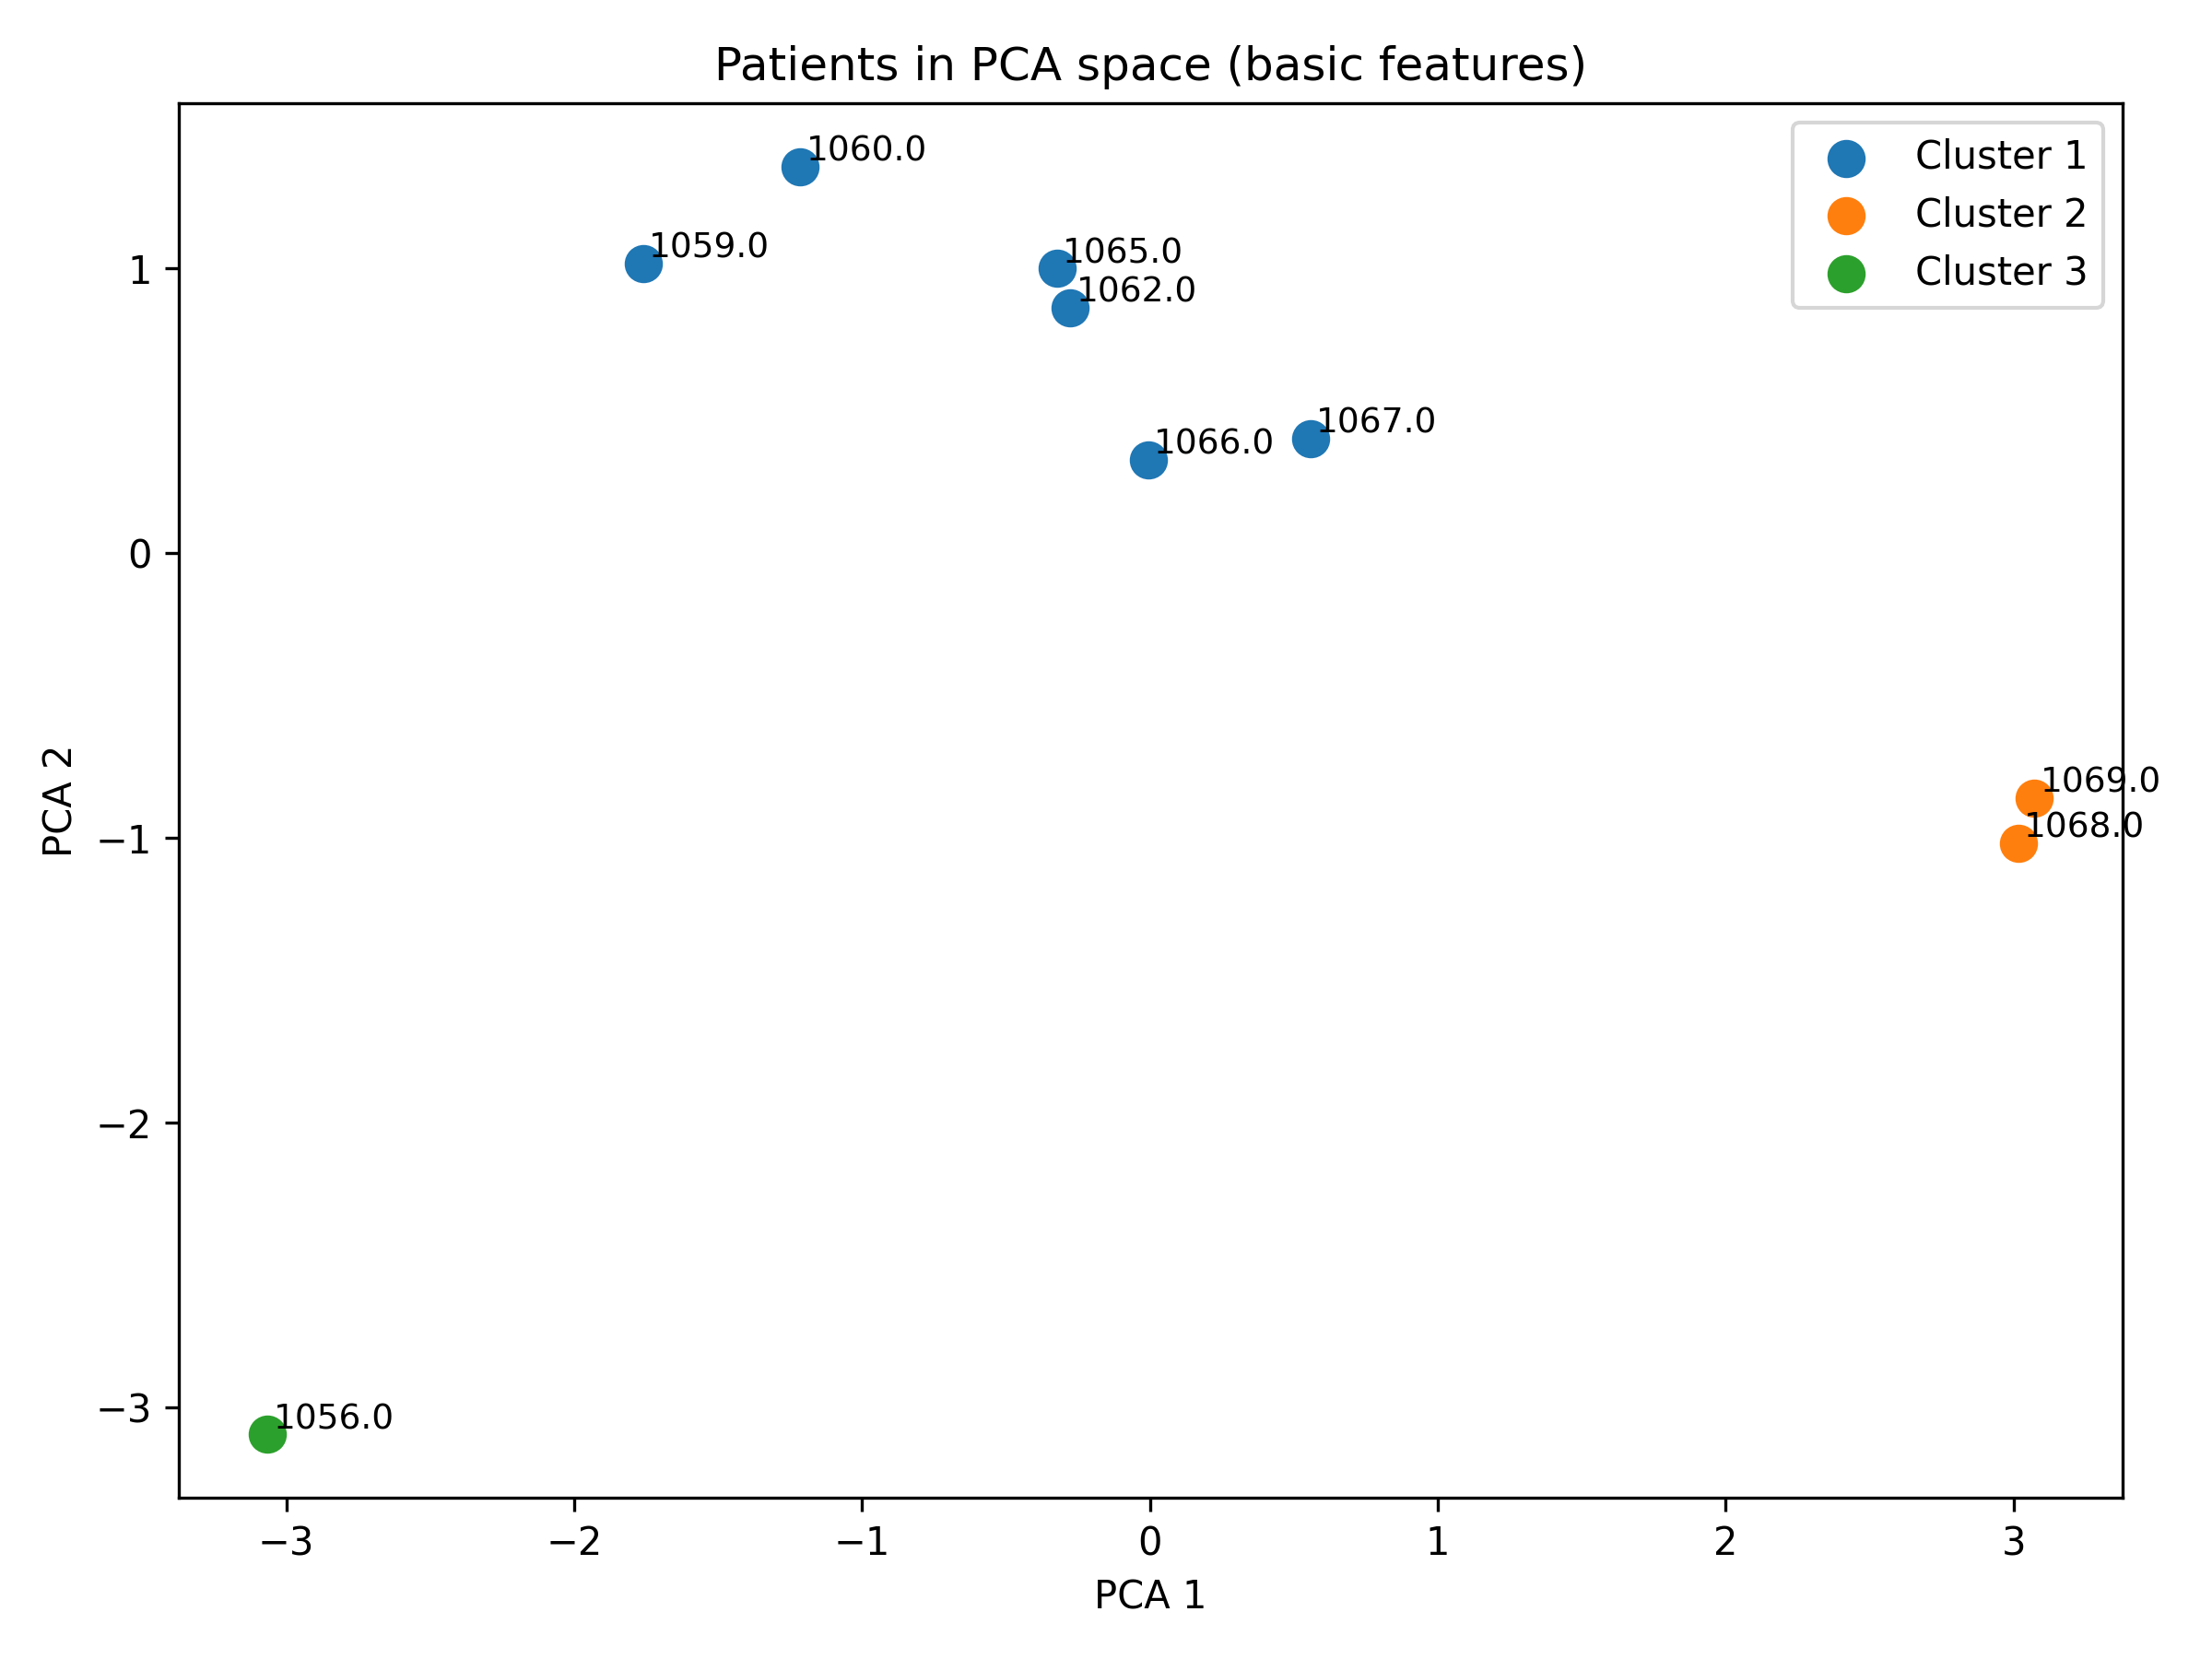
\includegraphics[width=0.7\textwidth]{patient_pca_clusters.png}
    \caption{Patients represented in the first two principal components (PCA1 and PCA2) of the image-derived features. Each point corresponds to one patient and is coloured according to the unsupervised cluster assignment. Patient IDs are shown as labels next to the points.}
    \label{fig:patient_pca_clusters}
\end{figure}
